\section{Server Communication}
In order to communicate with the server we created an abstract class which must be inherited for each different request we make to the server. The class inherits from \inline{AsyncTask} which makes it easy to create a new task on a new thread and send the result to the \ac{ui} thread.

\begin{figure}[H]
\centering
\includegraphics[width=0.7\linewidth, page=2]{img/servercomtask.pdf}
\caption{ServerComTask}
\label{fig:servercomtask}
\end{figure}
\inline{ServerComTask} is a generic class, it declares a type which the abstract method \inline{ParseJson()} must return. The object retuned by \inline{ParseJson()} is created by parsing the JSON it is supplied with.

\inline{ServerAlertDialog} is a simple interface which just returns an \inline{AlertDialog} which the \inline{ServerComTask} can use to display an alert if something went wrong. The interface is suppose to be implemented by activities so all server requests can share the \inline{AlertDialog} reference. We use it to display a static message that notifies the user that the connection with the server failed.

\inline{OnResponseListener} is a generic interface. It is used by \inline{ServerComTask} to communicate the result to where the server request was started. It sends the generic type as the result with \inline{onResponse()}. If anything went wrong with the request and no answer was produced, then \inline{onFailed()} is called so the lack of a result can be handled.

We have several different request we can make from the application to the server:
\begin{description}
\item[FavouriteCom] Gets or sets whether a recipe is favourited by a specific user.
\item[FavouriteListCom] Gets the list of favourites for a specified user.
\item[IngredientCom] Gets a list of all ingredients so the user can use them to search for recipes by ingredients.
\item[IngredientSearchCom] Searches for recipes based a user specified ingredients.
\item[RecipeCom] Gets an entire recipe.
\item[RecipeSearchCom] Searches for recipes based on a user specified text string.
\end{description}

\begin{lstlisting}[language=java, label=lst:servercomtask, caption={Simplified code of the \inline{ServerComTask}}]
public abstract class ServerComTask<T> extends AsyncTask<String, Integer, T> {
    private ServerAlertDialog serverAlertDialog;
    private OnResponseListener<T> onResponseListener;

    protected abstract T parseJson(String json) throws Exception;
    
    public ServerComTask(String apiPath, ServerAlertDialog serverAlertDialog, OnResponseListener<T> onResponseListener) {
    
        this.apiPath = apiPath;
        this.serverAlertDialog = serverAlertDialog;
        this.onResponseListener = onResponseListener;

        this.execute(apiPath);
    }

    @Override
    protected T doInBackground(String path) {
        try {
            String response = this.download(path);
            return this.parseJson(response);
        } catch (Exception e) {
            return null;
        }
    }

    @Override
    protected void onPostExecute(T result) {
        if (result == null) {
            this.onFailed();
            return;
        }
        this.onResponseListener.onResponse(result);
    }
    
    private void onFailed() {
        this.onResponseListener.onFailed();
        this.showAlertDialog();
    }
}
\end{lstlisting}

\begin{description}
\item[Lines 7-14] The constructor for \inline{ServerComTask}. It must have a \inline{ServerAlertDialog} to display errors, and it must have an \inline{OnResponseListener} to send the result to.
\item[Line 13] The call to \inline{execute()} starts the overriden abstract method \inline{doInBackground()} on a new thread. We chose to execute the task when the class is instantiated, since the task can only be executed once per instance of the task, so it is required that the path to download from is specified in the constructor.
\item[Lines 16-24] \inline{doinBackground()} must return the generic type. The result is then passed to the method \inline{onPostExecute()} which runs on the \ac{ui} thread.
\item[Line 19] First we download the data from the server. The download is an \textit{http get} request, so any parameters to the call is specified in the path. The \inline{download()} method is not shown.
\item[Line 20] The the response JSON is parsed to the generic type and returned to the \ac{ui} thread.
\item[Lines 28-31] If the result of the task is \inline{null} then the task failed. \inline{onFailed()} handles this.
\item[Line 32] The generic type result is sent to the response listener, and the execution of the task is complete.
\item[Lines 35-38] If the task failed, then we notify the \inline{OnResponseListener} that the task failed and we show an alert to the user.
\end{description}
The different server request implementations are not shown, they only specify a generic type and then parse the supplied JSON to the generic type. An example of how to make a request on the server and then handle the response is shown in \autoref{lst:recipesearchcom}. It is easiest to create an in line implementation of the \inline{OnResponseListener} interface, but you need to make sure to get the generic types right. Luckily the Android Studio \ac{ide} \todo{acronym overkill?} can generate the correct \inline{OnResponseListener} for us.\todo{er det Android Studio eller IntelliJ der genererer?}

\begin{lstlisting}[language=java, label=lst:recipesearchcom, caption={Search for recipes by text}]
new RecipeSearchCom((ServerAlertDialog) this.getActivity(), query, new OnResponseListener<ArrayList<IntermediateRecipe>>() {
    
    @Override
    public void onResponse(ArrayList<IntermediateRecipe> result) {
        RecipeSearchFragment.this.displayRecipeList(result);
        RecipeSearchFragment.this.progressCircle.setVisibility(View.GONE);
    }

    @Override
    public void onFailed() {
        RecipeSearchFragment.this.progressCircle.setVisibility(View.GONE);
    }
});
\end{lstlisting}

\begin{description}
\item[Line 1] We make a new instance of \inline{RecipeSearchCom} and create an in line implementation of the \inline{OnResponseListener}. Both the class and the interface uses the generic type \inline{ArrayList<IntermediateRecipe>} which is the result of the request. An \inline{IntermediateRecipe} is a partial recipe, used to display recipe search results. When the user wants to view the recipe, then the entire recipe is download. \todo{Der skal måske være en forklaring af vores applikation model før det her hvor det bliver forklaret} A \inline{query} string is specified which is the recipe text to search for.
\item[Lines 5-6] When the request is done we display the recipe search results in \inline{RecipeSearchFragment.this}, and hide the progress circle.
\item[line 11] If the request failed then we must make sure to hide the progress circle as well, the \inline{ServerComTask} will show an alert to the user.
\end{description}
